%\documentclass[12]{article}
%%%%%%%%%%%%%%%%%%%%%%% file template.tex %%%%%%%%%%%%%%%%%%%%%%%%%
%
% This is a general template file for the LaTeX package SVJour3
% for Springer journals.          Springer Heidelberg 2010/09/16
%
% Copy it to a new file with a new name and use it as the basis
% for your article. Delete % signs as needed.
%
% This template includes a few options for different layouts and
% content for various journals. Please consult a previous issue of
% your journal as needed.
%
%%%%%%%%%%%%%%%%%%%%%%%%%%%%%%%%%%%%%%%%%%%%%%%%%%%%%%%%%%%%%%%%%%%
%
% First comes an example EPS file -- just ignore it and
% proceed on the \documentclass line
% your LaTeX will extract the file if required
\begin{filecontents*}{example.eps}
%!PS-Adobe-3.0 EPSF-3.0
%%BoundingBox: 19 19 221 221
%%CreationDate: Mon Sep 29 1997
%%Creator: programmed by hand (JK)
%%EndComments
gsave
newpath
  20 20 moveto
  20 220 lineto
  220 220 lineto
  220 20 lineto
closepath
2 setlinewidth
gsave
  .4 setgray fill
grestore
stroke
grestore
\end{filecontents*}
%
\RequirePackage{fix-cm}
%
%\documentclass{svjour3}                     % onecolumn (standard format)
%\documentclass[smallcondensed]{svjour3}     % onecolumn (ditto)
\documentclass[smallextended]{svjour3}       % onecolumn (second format)
%\documentclass[twocolumn]{svjour3}          % twocolumn
%
\smartqed  % flush right qed marks, e.g. at end of proof
%
\usepackage{graphicx}
\usepackage{times}
\usepackage{natbib}
\usepackage{multicol}
\usepackage{hyperref}
%\usepackage[justification=centering]{caption}
%\usepackage{subcaption}

\usepackage{amsmath, amssymb, fullpage, array, algorithm2e,graphicx,mathtools, xparse}

\usepackage{color}
\usepackage{subfigure}
%\usepackage{mathabx}
%\usepackage[dvips]{graphics}
\newtheorem{thm}{Theorem}[section]
\newtheorem{dfn}{Definition}[section]
\newtheorem{cor}{Corollary}[thm]
\newtheorem{con}{Conjecture}[thm]
%\setlength{\parindent}{0in}   % for no indent

\newcommand{\blue}{\color{blue}}
\newcommand{\red}{\color{red}}
\newcommand{\blX}{\mbox{\boldmath {\bf X}}}
\newcommand{\blS}{\mbox{\boldmath {\bf S}}}
\newcommand{\blB}{\mbox{\boldmath {\bf B}}}
\newcommand{\blW}{\mbox{\boldmath {\bf W}}}
\newcommand{\blU}{\mbox{\boldmath {\bf U}}}
\newcommand{\blY}{\mbox{\boldmath {\bf Y}}}
\newcommand{\blA}{\mbox{\boldmath {\bf A}}}
\newcommand{\blI}{\mbox{\boldmath {\bf I}}}
\newcommand{\blZ}{\mbox{\boldmath {\bf Z}}}


\topmargin -0.10in   % when making pdf
\textheight 8.5in  % when making pdf


%\newcommand{\b}[1]{\mathbf{#1}}


\begin{document}

\title{Using Visual Statistical Inference to Better Understand High Dimension, Low Sample Size Data}\label{ch:largepsmalln}
\vspace{-0.8cm}
\author{Niladri Roy Chowdhury \and 
Dianne Cook \and
Heike Hofmann \and
Mahbubul Majumder \and
Eun-Kyung Lee \and
Amy L. Toth}

\institute{Niladri Roy Chowdhury, Dianne Cook, Heike Hofmann, Mahbubul Majumder \at
              Department of Statistics, Iowa State University, Ames, IA, USA \\
              \email{niladrir@iastate.edu, dicook@iastate.edu, hofmann@iastate.edu, mahbub@iastate.edu}        
           \and
           Eun-Kyung Lee \at
           Department of Statistics, EWHA Womans University, Seoul, Korea\\
           \email{lee.eunk@gmail.com}
           \and 
           Amy L. Toth \at
           Departments of Ecology, Evolution, and Organismal Biology and Entomology, Iowa State University, Ames, IA, USA \\
           \email{amytoth@iastate.edu}
}

\date{Received: date / Accepted: date}

\maketitle

\begin{abstract}
Statistical graphics play an important role in exploratory data analysis, model checking and diagnosis. With high dimensional data, this often means plotting low-dimensional projections, for example, in classification tasks projection pursuit is used to find low-dimensional projections that reveal differences between labelled groups. In many contemporary data sets the number of observations is relatively small compared to the number of variables, which is known as a high dimension low sample size (HDLSS) problem. This paper explores the use of visual inference on understanding low-dimensional pictures of HDLSS data. Visual inference helps to quantify the significance of findings made from graphics.  This approach may be helpful to broaden the understanding of issues related to HDLSS data in the data analysis community. Methods are illustrated using data from a published paper, which erroneously found real separation in microarray data, and with a simulation study conducted using Amazon's Mechanical Turk.

\keywords{statistical graphics \and lineup \and visualization \and projection pursuit \and data mining}
\end{abstract}

\section{Introduction} 

Many problems needing solutions today require the analysis of data where more variables are measured than there are samples taken. This is commonly referred to as high dimensional, low sample size (HDLSS) data (see for e.g. \cite{hall:2005}).   
HDLSS data occur in many application areas like face recognition, spectroscopy  and gene expression analysis. Classical statistical methods often fail in this context, because of insufficient data to support for parameter estimation. 

Reducing the dimension, using principal component analysis (PCA), would be a classical first step in the analysis of HDLSS data. PCA requires estimating the eigenvalues (maximum variance) and eigenvectors (direction of maximum variance) of the population variance-covariance based on the sample. With insufficient data this is a Sisyphean task. Just imagine, estimating a line on the foundation of a single point - there are infinitely many possibilities for lines. For classification tasks, finding a low-dimensional space where the classes are separated is a common first step. Linear discriminant analysis (LDA) is the classical approach. LDA solves an eigenvalue decomposition problem comparing distances between group means with variance around each mean. Estimating the variance-covariance is problematic when there are few points. In addition, when there are few sample points in high dimensions, differences between groups can be found in many different low-dimensional spaces, simply because of the sparseness of space.

\cite{marron:2007} describes the estimation issues associated with HDLSS.  
%One of the problems with HDLSS data is that not all the measured variables are ``important'' for understanding the underlying phenomenon of interest. 
Advancements in PCA to handle HDLSS data have been done by \cite{marron:2011} and \cite{yata:2010}. \cite{donoho:2009} and \cite{donoho:2008} study optimal variable selection and introduce a principle of model selection for problems where where only a small fraction of the variables are useful and unknown. Penalization is another common approach to handle HDLSS, and has been applied to classification problems \citep[e.g.][]{witten:2011, lee:2009}. Estimates of the variance-covariance are obtained by an interpolation with the identity matrix, effectively reducing the importance of some variables. 

So, although substantial research has produced many new approaches to creating better models and estimation for HDLSS data, the major issues are still not clear to many data analysts. For example, \cite{toth:2010} make a common mistake of seeing structure where none exists. Figure \ref{oligo} reproduces the result in this paper.  They use LDA to examine gene expression data of wasps containing 447 variables and 50 cases. There are 50 different paper wasps divided into 4 types: Foundress (F), Gyne (G), Queen (Q) and Worker (W), 14  wasps of type Foundress and 12 each of the other 3 types. The authors, knowing that LDA requires that the dimension ($p$) should be smaller than the number of observations ($n$), first reduced the dimension from 447 to 40 by randomly selecting a subset of significantly different oligonucleotides. LDA produced a 2D projection ($d=2$) of best separation. This is almost the same approach as used in \cite{dudoit:2002}, one of the first studies of classification of gene expression data. What results is a picture of the four groups that suggests big differences in the types of wasps. There exists no conventional inferential methods which enables us to conclude whether this apparently clear separation is statistically significant or not. For prediction, typically data is broken into training and test sets, or cross-validation is conducted to assess the significance of difference, using test set error. This approach does not work well for visualization.

\begin{figure*}[hbtp]
   \centering
       \scalebox{.45}{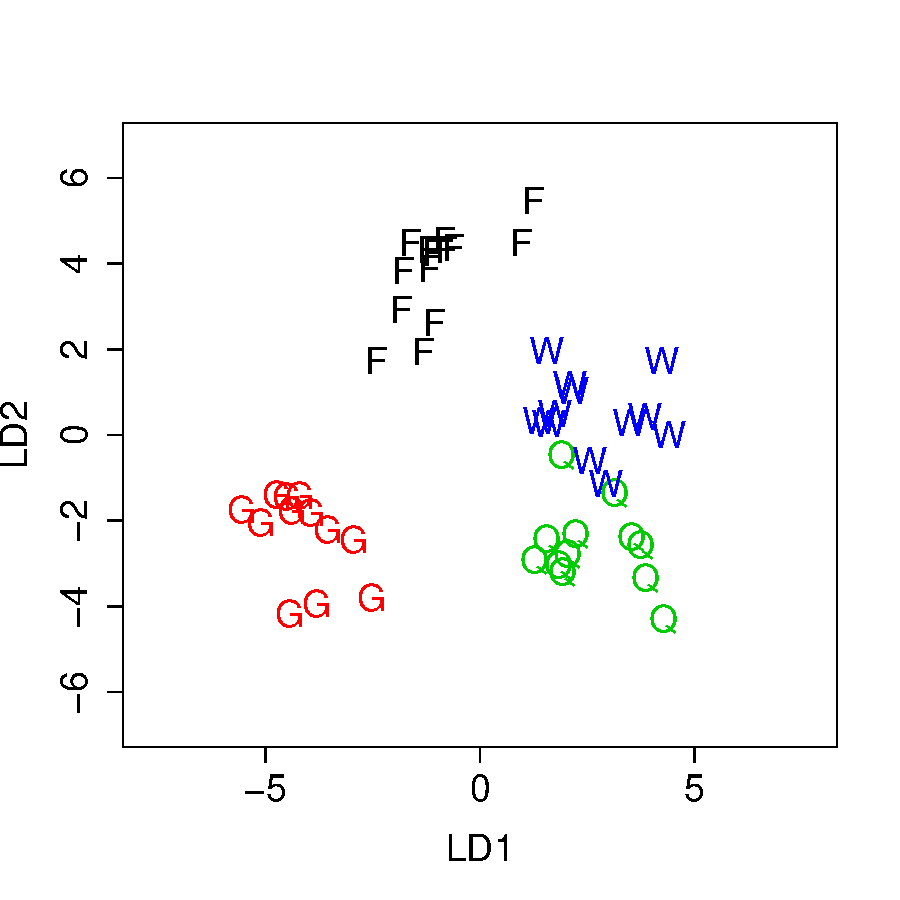
\includegraphics{toth_lda.pdf}}
       \caption{LD1 versus LD2 from an LDA on a randomly selected subset of 40 significantly different oligos : F, Foundress; G, gyne; Q, queen and W, worker. It can be noticed that the groups F and G are separated. This plot is generated to match Figure 2 in \cite{toth:2010}. }
     \label{oligo}
\end{figure*}  

We propose that new methods for inference on graphics might be helpful for building understanding very generally. Visual statistical inference was first conceptually introduced by \cite{buja:2009}, formalized and validated by \cite{majumder:2013}. Using visual inference, it can be shown that there is no real difference between the wasp groups - what you see is a mirage. 

Visual inference may also be useful in related applications, such as checking algorithms that produce visual results. We used the approach described in this paper to check the optimization algorithm of projection pursuit in the \texttt{tourr} package \citep{tourr:2011} in \texttt{R} \citep{r}. The optimization procedure was new, and we suspected that it was being sensitive to the order of data values, and returning projections of purely noise data that we thought were surprisingly distinct from noise. Visual inference was able to temper our concerns.   

This paper describes visual statistical inference as applied to dimension reduction for HDLSS. In particular we focus on dimension reduction using projection pursuit, and the effect that having high dimension has on the robustness of the separation between groups.  Small simulation experiments are used to examine the problem in a controlled setting. The next section explains visual inference methods. Section \ref{sec:dimred} discusses the dimension reduction methods. Section \ref{sec:turk} describes Amazon's Mechanical Turk  \citep{turk}  which was used to conduct the experiment. The application of visual inference methods on wasp data is described in Section \ref{sec:wasp}. Section \ref{sec:experiment} discusses the experiment designed to examine people's perception of separation in the presence of real separation and ``purely noise'' for simulated HDLSS data. Section \ref{sec:results} discusses the collected data and results. 


\section{Visual inference methods} \label{sec:inference}

\cite{buja:2009} proposed two protocols, the Rorschach and the lineup. While the Rorschach protocol helps to understand the extent of randomness, the lineup protocol is  used for testing significance of findings. These methods together are called visual statistical inference. \cite{majumder:2013} made a head-to-head comparison between visual statistical inference tests and classical tests which showed that the lineup protocol performs similarly to the classical tests. Unlike classical hypothesis testing, the test statistic in visual inference is not numeric, but a plot that is appropriately chosen to display a  distinctive pattern in case that the null hypothesis is false. The lineup protocol of size $m$ embeds the observed data plot amongst ($m$ - 1) null plots. Null plots are created by a mechanism consistent with the null hypothesis. Human subjects are asked to identify the plot in the lineup with the most distinct feature(s). When the alternative hypothesis is true, it is expected that the plot of the observed data, the test statistic, will have visible feature(s) inconsistent with the null hypothesis. If the subjects choose the plot of the observed data, this is evidence against the null hypothesis and with enough support, the null hypothesis is rejected. 

An illustration of the lineup protocol in contrast to the conventional test is shown in Table \ref{tbl:compare}. Both start with the same hypothesis but the test statistic in a conventional setting is the parameter estimate divided by its standard error. In visual inference the test statistic is a plot of the observed data. In this case, a dot plot is used since the variable of interest is continuous with two groups. In a conventional test the value of the test statistic is compared with all possible values of the sampling distribution, the distribution of the test statistic if the null hypothesis is true. If it is extreme, then the null hypothesis is rejected. In visual inference, the plot of the data is compared with a finite number of samples drawn from the sampling distribution. If the actual data plot is selected as the most different, then the null hypothesis is rejected. 

\begin{table*}[hbtp]
\centering 
\caption{Comparison of visual inference with traditional hypothesis testing. Starting with the same hypothesis, the test statistic in a conventional setting is a real number while in visual inference it is a plot of the observed data. In conventional test the value of the test statistic is compared with all possible values of the sampling distribution. $H_o$ is rejected if it is extreme. In visual inference, the plot of the data is compared with a finite number of samples drawn from the null distribution. If the actual data plot is identifiable, then the null hypothesis is rejected. 
}
\begin{tabular}{llll} 
\hline
  & Mathematical Inference &  Visual Inference \\ 
\hline
  Hypothesis & $H_o: \mu_1= \mu_2$ vs $H_a: \mu_1 \ne \mu_2$& $H_o: \mu_1 = \mu_2$ vs $H_a: \mu_1 \ne \mu_2$\\
%  \vspace{0.5cm}	
 & \begin{minipage}[h]{1.5cm} \begin{center} \scalebox{0.25}{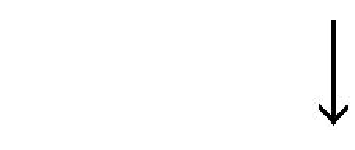
\includegraphics{down_arrow.pdf}} \end{center} \end{minipage} & \begin{minipage}[h]{1.5cm} \begin{center} \scalebox{0.25}{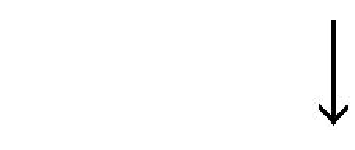
\includegraphics{down_arrow.pdf}} \end{center} \end{minipage} \\
%\vspace{0.5cm}				  
 Test Statistic & $T(y)=\frac{\overline{y}_1 - \overline{y}_2}{s\sqrt{\frac{1}{n_1} + \frac{1}{n_2}}}$ & $V(y)=$ \begin{minipage}[h]{1cm} \begin{center} \scalebox{0.35}{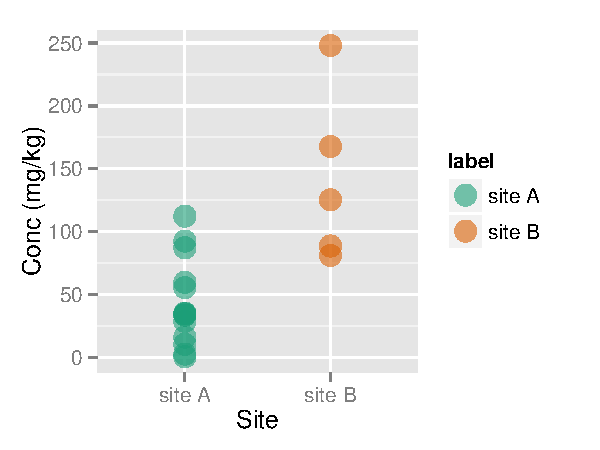
\includegraphics{data-dot-rev.pdf}} \end{center} \end{minipage} \\
				 
 & \begin{minipage}[h]{1.5cm} \begin{center} \scalebox{0.25}{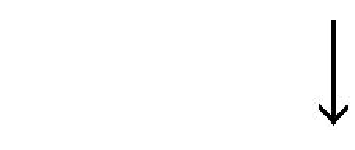
\includegraphics{down_arrow.pdf}} \end{center} \end{minipage} & \begin{minipage}[h]{1.5cm} \begin{center} \scalebox{0.25}{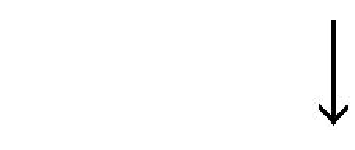
\includegraphics{down_arrow.pdf}} \end{center} \end{minipage} \\
				 
 Sampling Distribution & $f_{T(y)}(t); $\begin{minipage}[h]{1.5cm} \begin{center} \scalebox{0.5}{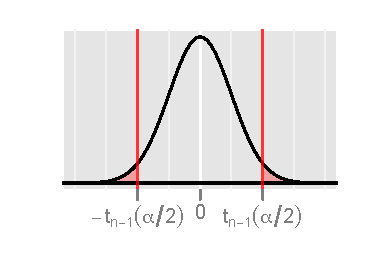
\includegraphics{two-sided-rejection.pdf}} \end{center} \end{minipage} & $f_{V(y)}(t); $ \begin{minipage}[h]{1.5cm} \begin{center} \scalebox{0.29}{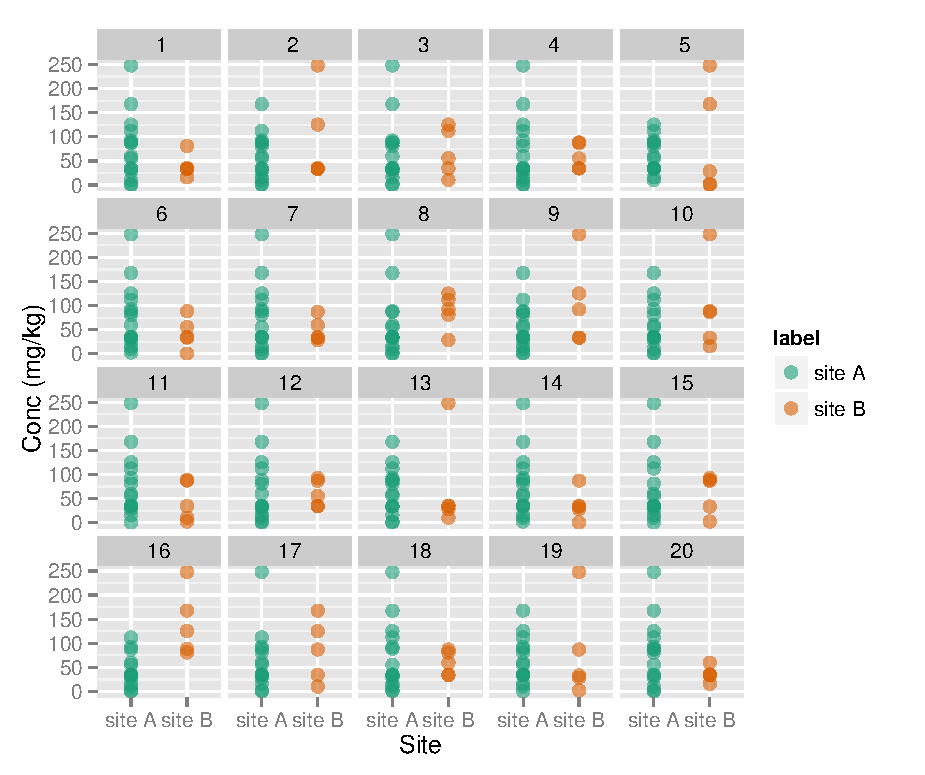
\includegraphics{lineup-dot-rev.pdf}} \end{center} \end{minipage} \\
 & \begin{minipage}[h]{1.5cm} \begin{center} \scalebox{0.25}{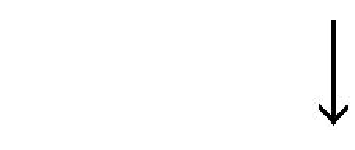
\includegraphics{down_arrow.pdf}} \end{center} \end{minipage} & \begin{minipage}[h]{1.5cm} \begin{center} \scalebox{0.25}{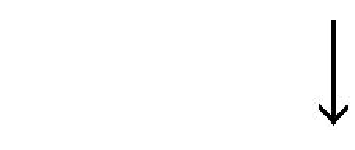
\includegraphics{down_arrow.pdf}} \end{center} \end{minipage} \\
 Reject $H_o$ if & observed $T$ is extreme & observed data plot is identifiable \\
\hline 
\end{tabular}
\label{tbl:compare}
\end{table*}


For example, suppose we have two sample data on the concentration of a metal in $mg/kg$ for sites A and B of sizes $n_1$ and $n_2$ respectively. We want to test whether there exists a difference between the concentration levels in the two sites A and B. To test for statistically significant difference between the two populations from which the data was sampled, let $\mu_1$ denote the mean concentration level in Site A and $\mu_2$ denote the mean concentration level in Site B. Thus the null and alternative hypothesis would be
\[
H_o: \mu_1 = \mu_2 \qquad \hbox{versus} \qquad H_a: \mu_1 \ne \mu_2
\]
The conventional test would be a two-sample t-test with test statistic $T(y)$ described in Table \ref{tbl:compare}. One way to plot this data is a side-by-side dotplot. Let this be the visual test statistics $V(y)$. Null plots are generated assuming that $H_o$ is true. Here, this is achieved by randomly permuting the site label. The observed data plot is placed randomly among the null plots to obtain a lineup. In this example, $m = 20$ is the size of the lineup - there are 19 null plots. If $H_o$ is not true, the dots of one group should be vertically shifted relative to the other group. If the human observer can identify the plot of the real data, there will be reason to believe that the observed data plot has a pattern which is absent in the null plots leading to a rejection of the null hypothesis. If the viewer cannot identify the observed data plot, we fail to reject the null hypothesis. Under the null hypothesis, each observer has a $1/m$ chance of picking the observed plot from a lineup of size $m$. Hence $1/m$ is the minimal value at which we can set the Type I error, $\alpha$, consistent with $\alpha = 0.05$ if $m = 20$.  \cite{majumder:2013} provides more detailed discussion about this. For this problem, visual inference enables the handling of the small sample size and non-normality of the population. However, in general the setting for visual inference would be problems where no conventional test exists.
\begin{figure}[hbtp]
   \centering
       \scalebox{1}{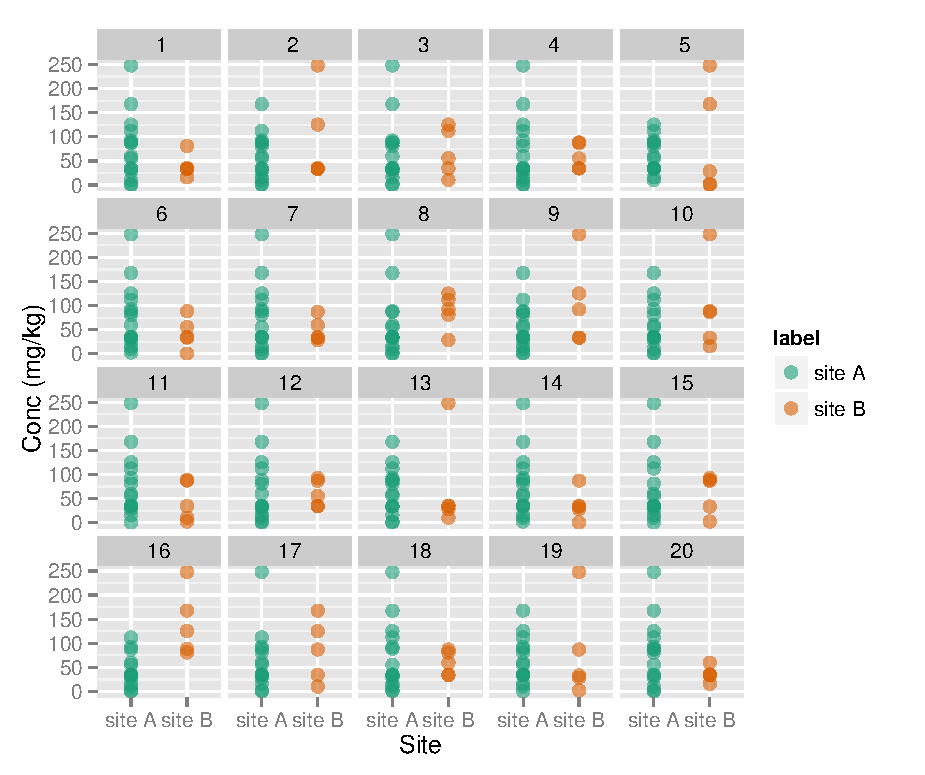
\includegraphics{lineup-dot-rev.pdf}}
      \caption{A typical lineup  ($m = 20$) for testing $H_o: \mu_1 =  \mu_2$. 
      When the alternative hypothesis is true, the observed data plot should have the largest vertical difference between the centers. Can you identify the observed data plot? The solution to the lineup is provided in the Appendix.}
      \label{lineup}
\end{figure}

\cite{majumder:2013} describes the methods of obtaining the power of the visual test, by combining results from multiple users. For their simulation experiments human observers were recruited through Amazon's Mechanical Turk \citep{turk}. Power of the visual test used in their simulation was also calculated theoretically. Their results suggest that the power of visual statistical inference is comparable to conventional tests in a setting of testing the parameters of linear regression models. The subject specific power of the visual test can also be estimated from the multiple responses data from each human observer, which might help quantify individual visual skills.

 
\section{Dimension reduction}  \label{sec:dimred}

Projection pursuit \citep[e.g.][]{friedman:1974}  is used for dimension reduction in our studies. Projection pursuit (PP) finds the most interesting low dimensional projection of high dimensional data by maximizing some criterion of interest, e.g. variance or clustering or group separation. As pointed out in \cite{huber:1985} the most exciting feature of projection pursuit is that it can bypass the curse of dimensionality. 

In classification problems, linear discriminant analysis (LDA) can be used to find a low-dimensional space where the groups are most separated. This corresponds to using the LDA index \citep{lee:2009} in projection pursuit. Let $\bf{X_{ij}}$ be the $p$-dimensional vector of the $j$th observation in the $i$th class, $i = 1, \dots, g, j = 1, \dots, n_i$, $g$ is the number of classes, $n_i$ is the number of observations in class $i$, and $n = \sum_{i = 1}^g n_i$. Let $\overline{\blX}_{i.} = \frac{1}{n_i} \sum_{j=1}^{n_i} \blX_{ij}$
be the $i$th class mean and $\overline{\blX}_{..} =
\frac{1}{n}\sum_{i=1}^g \sum_{j=1}^{n_i} \blX_{ij}$ be the total
mean. The LDA PP index is
\begin{equation}
I_{LDA} ({\blA}) = \left \{ \begin{array}{cc}
                       1-\frac{\big|{\blA}^T\blW{\blA}\big|}{\big|{\blA}^T\big
                                  (\blW + \blB\big){\blA}\big|} &
                       \mbox{ for $\big|{\blA}^T\big(\blW + \blB\big) {\blA}\big| \ne 0$}\\
                       0 & \mbox{for  $\big|{\blA}^T\big(\blW + \blB\big) {\blA}\big| = 0$}
                       \end{array}
               \right.
\end{equation}
where $\blA$ is an orthogonal projection onto a $k$-dimensional space and

\begin{eqnarray}
 \blB&=&\sum_{i=1}^g n_i (\overline{\blX}_{i.} - \overline{\blX}_{..})(\overline{\blX}_{i.}
  - \overline{\blX}_{..})^T
:  \mbox{between-class sums of squares}, \nonumber\\
\blW&=&\sum_{i=1}^g \sum_{j=1}^{n_i} (\blX_{ij} -
\overline{\blX}_{i.})(\blX_{ij} - \overline{\blX}_{i.})^T :
\mbox{within-class sums of squares}.\nonumber
\end{eqnarray}

For HDLSS data, the penalized discriminant analysis (PDA) index \citep{lee:2009} is more robust. Let ${\blX}_{ij}^*$ be the standardized vector of ${\blX}_{ij}$. Then 

\begin{eqnarray}
 \blB^s&=&\sum_{i=1}^g n_i (\overline{\blX}^*_{i.} - \overline{\blX}^*_{..})(\overline{\blX}^*_{i.}
  - \overline{\blX}^*_{..})^T: \hbox{between-class sums of squares of the standardized data}\nonumber\\
\blW^s&=&\sum_{i=1}^g \sum_{j=1}^{n_i} (\blX^*_{ij} -
\overline{\blX}^*_{i.})(\blX^*_{ij} - \overline{\blX}^*_{i.})^T: \hbox{within-class sums of squares of the standardized data }\nonumber
\end{eqnarray}
where $\overline{\blX}^*_{i.}$ is the $i$th class mean of the standardized data and $\overline{\blX}^*_{..}$ is the
total mean of the standardized data, which is 0. The PDA index is defined as

\begin{eqnarray}
I_{PDA}(\blA,\lambda) =
1-\frac{\Big|\blA^T\big\{(1-\lambda)\blW^s+n\lambda\blI_p\big\}
\blA\Big|}
              {\Big|\blA^T\big\{(1-\lambda)(\blB^s +\blW^s)+n\lambda\blI_p\big\} \blA\Big|}\label{PDA3}
\end{eqnarray}
where $\blA$ is an orthonormal projection onto a $k$-dimensional space
and $\lambda \in [0,1)$ is a predetermined parameter. Penalized LDA \citep{witten:2011} is a similar approach.

These indices are available for projection pursuit using the \texttt{tourr} package \citep{tourr:2011} in \texttt{R} \citep{r}. The \texttt{tourr} package produces tours of multivariate data. The package also includes functions for creating different types of tours like grand, guided and little tours, which project multivariate data with $p$ dimensions to 1, 2, 3 or $d$ dimensions where $d \le p$. The guided tour function is used here. The guided tour will converge to a maximally interesting projection. Here, that is a projection where groups show the biggest separation. For this paper we used $d = 1$ or 2.  

\section{Amazon Turk experiments} \label{sec:turk}

Amazon's Mechanical Turk \citep{turk} is a service that enables researchers to employ people to do tasks which computers perform poorly. In exchange of their efforts, the subjects are paid, not substantially, but on the scale of the minimum wage of the USA. For visual inference studies, subjects are typically given a block of ten lineups to evaluate during a job. From this block, one lineup is typically used as a filter, and the remaining lineups produce data for the studies. Because a subject evaluates more than one lineup, and a lineup is evaluated by more than one subject, we obtain some replication in the results upon which to estimate variation. The one filter lineup, in which the observed data plot is markedly different from the nulls, is necessary because Turkers are not manually monitored, and a few attempt to maximize financial gain without taking the exercise seriously. 

For this paper, two Turk studies were run, one for the wasps data, and the other for the simulation study. Turkers are redirected from Amazon to a website which describes the study in detail, provides some practice trials, collects demographic details, and responses. The website of the simulation study is \url{http:/mahbub.stat.iastate.edu/feedback_turk7/homepage.html}.

\section{Wasps application} \label{sec:wasp}

We return to the motivating example. Figure \ref{oligo} suggested that the expression patterns of the wasp groups are different.  The question of interest is ``Is this separation real?'' This can be investigated by testing the hypothesis: 

\begin{quote}
$H_o$: There is NO difference in the expression levels between the types of wasp.\\
$H_a$: At least one of the types of wasps has different expression levels.
\end{quote}
A lineup is made of the wasp data obtained from \cite{toth:2010} to test $H_o$ where the null plots are made by permuting the wasp type label, and re-doing the LDA. If there is a real difference between the expression levels for the types of wasps then the observed data plot should be detectable in the lineup. Figure \ref{toth_lineup} shows a lineup.  Three different lineups were created using this procedure. 

\begin{figure*}[hbtp]
%\begin{figurehere}
   \centering
       \scalebox{1.00}{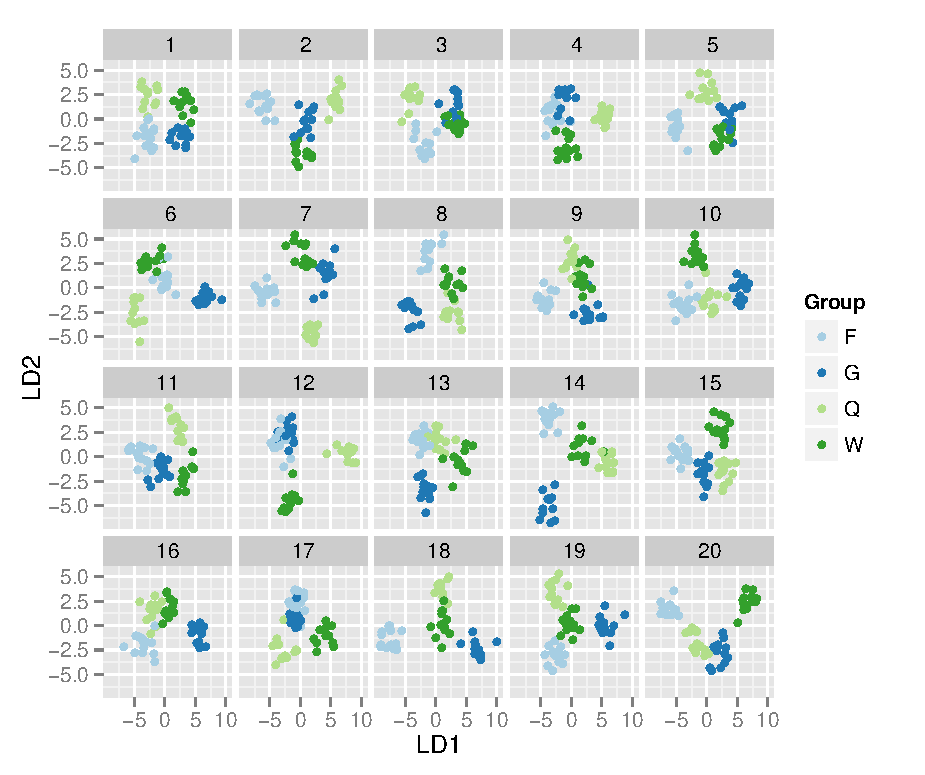
\includegraphics{lineup-wasp-8-rev.pdf}}
       \caption{Lineup of the wasps data. One plot shows the observed data and the remaining 19 show null data where the wasp type labels were randomly assigned. Each plot was produced by conducting LDA on the 40D data to produce the 2D projection with best separation. Which plot shows the most separation between the 4 groups? The solution is provided in the Appendix.}
       \label{toth_lineup}
\end{figure*} 

In addition, three more lineups are made containing only null plots, with one plot randomly chosen to act as an observed data plot. These lineups were shown to the subjects recruited from Amazon Turk.  A total of 116 subjects evaluated the 6 lineups. Table \ref{wasp} shows the results. The success rate in detecting the plot of the wasp data is 0! This is worse than that of purely noise data. You will notice that for one of the purely noise lineups, subjects very often correctly picked the (random) observed data plot. This happened because the randomly generated observed data plot actually had more separation than any other plot in that lineup. This is the nature of randomness, but makes for interesting results here. The $p$-value is calculated according to the procedure given by \cite{majumder:2013}. The large $p$-values indicate that there is no statistically significant evidence upon which we reject the null hypothesis. Thus we have to conclude that the separation in the wasp data is not real. It is purely the effect of high dimensionality. 

\begin{table}[ht]
\begin{center}
\caption{Results of the Turk study on the wasps data. Proportion correct for each lineup is shown, with the number of subjects, and $p$-value associated. The success rate is highest for one of the purely noise lineups, which occurred because the plot with the most difference between groups happened to be the one that is randomly generated as the ``real'' data. Averaging the $p$-values for each set of lineups, for the wasps is 1.0, and for the pure noise, is 0.67 suggesting that the apparent separation in the wasp data is consistent with pure noise induced by the high dimensions.}
\vspace{0.15cm}
\begin{tabular}{r|r|r|rr}
\hline
  \hline
 Data & Replicate & Num Subjects & Prop Correct & $p$-value\\ 
  \hline
  & 1 & 25 & 0.0000 &  1.0000\\
Wasps & 2 & 13 & 0.0000 &  1.0000\\ 
 & 3 & 27 & 0.0000 &  1.0000\\
 \hline
 & 1 & 19 & 0.2632 &  0.0002\\
Purely noise & 2 & 18 & 0.0000 &  1.0000 \\ 
 & 3 & 14 & 0.0000 &  1.0000\\
   \hline
\end{tabular}
\label{wasp}
\end{center}
\end{table}

The probability of separation by chance between two groups in purely noise data, given a fixed sample size and dimension,  was quantified by \cite{ripley:1996} (Proposition 3.1). Figure \ref{dist_1d} illustrates this result for 1D projections, for different $p$, where sample size is fixed at $n = 30$. When $p = 2$, $\hbox{P(separation}|n = 30, p = 2) = 0$ and it reaches 1 when $p = 25$. For data of the size of the wasps, $n = 50$ and $p = 38$, the probability of obtaining separation with only two groups is 1, so we would expect that there would certainly be separation between four groups in 2D.

\begin{figure}[htbp]
\centering
\mbox{\subfigure[P(sep$|n,2$) = 0.00]{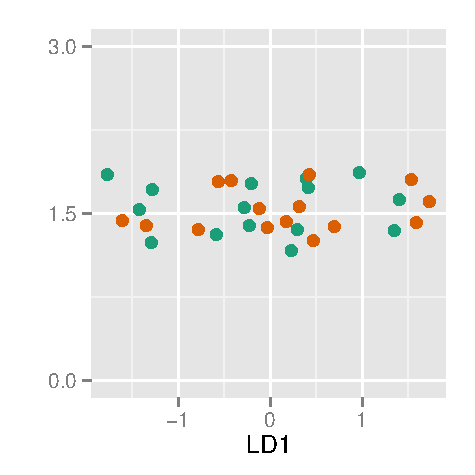
\includegraphics[width=1.1in]{noise-2-rev.pdf}}\quad
\subfigure[P(sep$|n,8$) = 0.01]{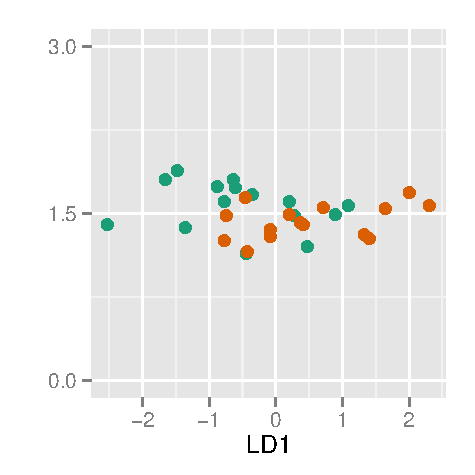
\includegraphics[width=1.1in]{noise-8-rev.pdf} }\quad
\subfigure[P(sep$|n,15$) = 0.64]{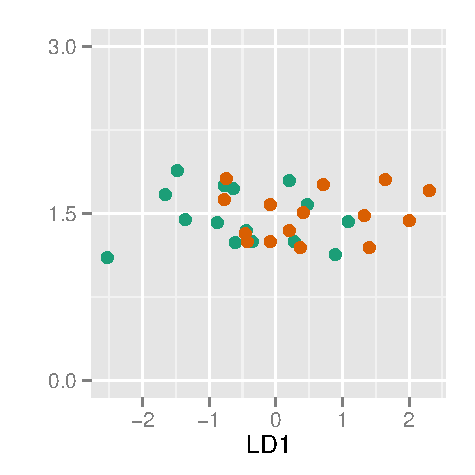
\includegraphics[width=1.1in]{noise-15-rev.pdf} }\quad
\subfigure[P(sep$|n,22$) = 0.99]{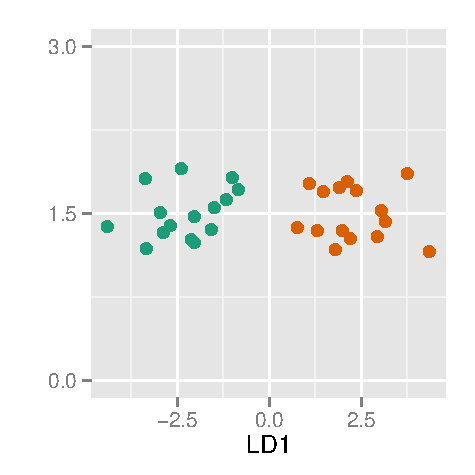
\includegraphics[width=1.1in]{noise-22-rev.pdf} }\quad
\subfigure[P(sep$|n,28$) = 1.00]{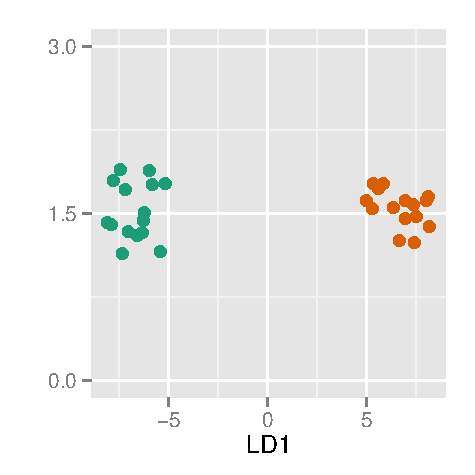
\includegraphics[width=1.1in]{noise-28-rev.pdf} }}
\caption{Plots showing example 1D projections for $p=2, 8, 15, 22, 28$ and $n = 30$. The probability of obtaining a projection where groups are separated is calculated and displayed below the plots. Of course, once a projection is computed the groups are either separated or not - the event occurred or didn't - and we can see that the last two plots display separated groups. The difference between the groups increases as $p$ increases, and the likelihood of obtaining a projection with separation increases.} 
\label{dist_1d}
\end{figure}

In the original paper \citep{toth:2010}, the dimensionality was reduced from 389 by choosing the genes that showed the greatest separation. So the problem of high dimensionality is actually even worse for these data. In general, reducing the data dimensions so that the sample size is bigger than dimension is not, on its own, sufficient. It is important, even, with so few cases to do cross-validation, or break the sample into training and test sets before conducting analysis. LDA is known also to be a problem for HDLSS data, because it requires estimating more parameters than the available data allows. A better prospect for dimension reduction is the penalized discriminant analysis (PDA) index \citep{lee:2009}, which helps adjust for the over-estimation. Other results and the overall conclusions in \cite{toth:2010} are not affected by the inadequacy revealed by this visual inference analysis. A similar LDA performed on wasp gene expression data with a much higher sample size in \cite{toth:2007} did not suffer from the HDLSS problem. We determined that there were robust separations between the groups based on those data (results not shown).


\section{Follow-up simulation experiment} \label{sec:experiment}

\subsection{Experimental design}

The goal is to determine how well people can detect the presence of real separation as distinguishable from random noise. To achieve this, the experiment is set up with several factors: real separation or pure noise, data dimension and projection dimension. Real separation is achieved by setting 1 or 2 variables with real separation among a number of noise variables.  Sample size is fixed to keep the experiment manageable. Also mean difference is kept fixed. The levels of the factors used in the experiment are given in Table \ref{freq}. Three replicates at each level are generated. These produced 60 different ``observed data sets'', and thus, 60 different lineups. 

\begin{table}[htbp]
\begin{center}
\caption{Levels of the factors used for the simulation experiment.}
\begin{tabular}{cccp{2.2cm}|c}
  \hline
  \hline
  $n$ & projection($d$) & separation & dimension ($p$) & replicates\\
  \hline
  30 & 1 & Yes & 20, 40, 60, 80, 100 & 3 \\
      & & No & 20, 40, 60, 80, 100 & 3\\
   30 & 2 & Yes & 20, 40, 60, 80, 100 & 3 \\
     & & No & 20, 40, 60, 80, 100 & 3\\   
      \hline
\end{tabular}
\label{freq}
\end{center}
\end{table} 

\subsection{Simulation process}

Two groups of $p$ dimensions of data with 15 observations in each group are generated from $N(0, 1)$.  The data from the first group is labeled as group 1 and the data from the second group as group 2, yielding a $30 \times (p + 1)$ matrix, ${\blX}$, is obtained where the first 15 observations are from group 1 and the last 15 observations are from group 2. The data for both the groups is purely noise, having no dependence on the groups. So ${\blX}$ can be written as
$${\blX}^{n \times (p + 1)} = ({\blX}_1, {\blX}_2, \dots, {\blX}_p, \hbox{Group})$$ where each ${\blX}_i$ is a vector of dimension 30 for $i = 1, \dots, p$. This matrix ${\blX}$ excluding the Group variable gives the $p$-dimensional pure noise data or data with no separation.

To introduce real separation in the data, values for $p$-th variable ${\blX}_p$ are shifted apart by 6 units between the two groups: 
$$
{\blX}_p = \left\{ \begin{array}{rl}
 {\blX}_p - 3 &\mbox{ if $ {\blX}_p \in$ group 1} \\
 {\blX}_p + 3 &\mbox{ if $ {\blX}_p \in$ group 2}
       \end{array} \right.
$$
and then standardized to have unit variance again. %Hence two sets of data are obtained, each with $p$ dimensions with $n = 30$ observations in each dimension divided into two groups. One of the datasets is pure noise and the other has some real separation in the $p$-th dimension. 
On each dataset of $p$ dimension, a projection pursuit optimization with the PDA index is performed to obtain the 1D projection of best separation, yielding $\blY = \blX \blA$.  

The above procedure is effectively the same for 2D projections with few key differences. The first 10 observations are labelled group 1, the second 10 observations as group 2 and the last 10 as group 3.  So, collectively,  ${\blX}$ can be written as
$$ {\blX}^{n \times (p + 1)} = ( {\blX}_1,  {\blX}_2, \dots, {\blX}_p, \hbox{Group})$$ where each $ {\blX}_i$ is a vector of dimension 30 for $i = 1, \dots, p$. This matrix ${\blX}$ excluding the Group variable gives the $p$-dimensional noise data or data with no separation with 3 groups.

To introduce real separation, the means of the 3 groups are adjusted in the last two dimensions i.e. $ {\blX}_{p-1}$ and ${\blX}_p$. The adjustment is done in the following way:
$$
( {\blX}_{p-1},  {\blX}_p) = \left\{ \begin{array}{rl}
 ( {\blX}_{p-1} - 3,  {\blX}_p) &\mbox{ if $( {\blX}_{p-1},  {\blX}_p) \in$ group 1} \\
 ( {\blX}_{p-1} + 3,  {\blX}_p) &\mbox{ if $({\blX}_{p-1},  {\blX}_p) \in$ group 2} \\
 ( {\blX}_{p-1} ,  {\blX}_p + \sqrt{27}) &\mbox{ if $( {\blX}_{p-1},  {\blX}_p) \in$ group 3}
       \end{array} \right.
$$
and standardized. If $ {\blX}_{p-1}$ versus ${\blX}_p$ are plotted in a scatterplot, the points cluster along the vertices of an equilateral triangle of side 6. Hence the data with 2 dimensions of real separation divided into 3 groups is obtained. A projection pursuit with a PDA index is performed to obtain the 2D projection of best separation, yielding ${\blY} = {\blX}{\blA}$. 

\subsection{Producing lineups}

Two different visual test statistics, $V_1({\blY})$ and $V_2({\blY})$ are used in this paper, for representing 1D and 2D data. $V_1({\blY})$ is a horizontal jittered dot plot, with color representing groups. $V_2({\blY})$ is a scatterplot with color representing groups. Symbols are kept constant for uniformity of appearance. Figure \ref{fig3} shows the two different visual test statistics.

\begin{figure}[htbp]
\centering
\mbox{\subfigure[$V_1({\blY})$]{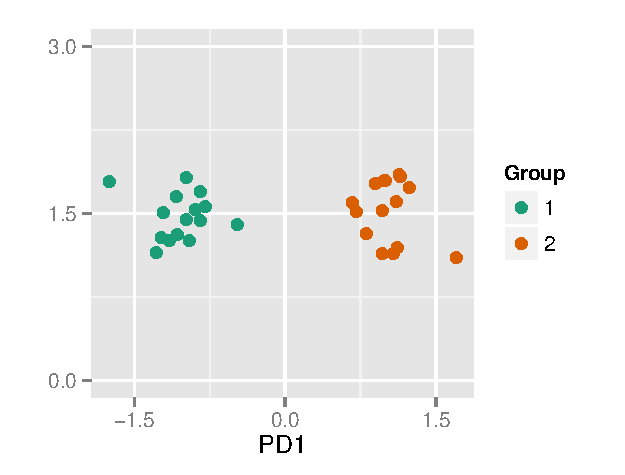
\includegraphics[width=2.5in]{test_statistic_1-rev.pdf}}\quad
\subfigure[$V_2({\blY})$]{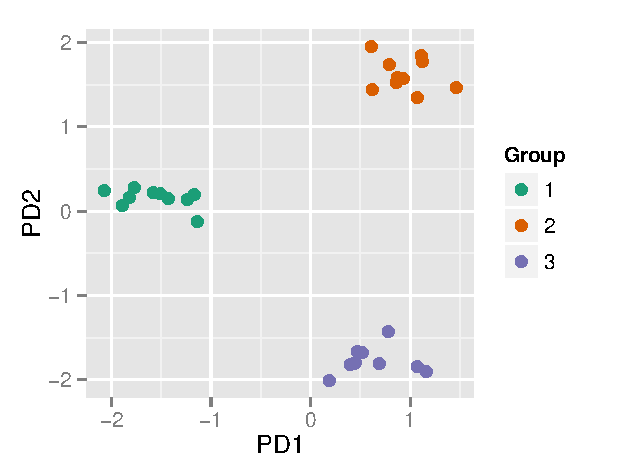
\includegraphics[width=2.5in]{test_statistic_2-rev.pdf} }}
\caption{The visual test statistics $V_1({\blY})$ and $V_2({\blY})$ used.  $V_1({\blY})$ is a horizontal jittered dot plot while $V_2({\blY})$ is a scatterplot of the first and second dimensional projections, with color representing groups in both cases. } 
\label{fig3}
\end{figure}

To obtain the null plots in a lineup, the group variable is permuted in order to break any dependence between the group variable and the other variables. Projections are obtained and plotted in the same way as the test statistic. The test statistic, which is the observed data plot, is placed randomly among the 19 null plots. To maintain the same orientation of the two groups in the 1D projection lineup,  the mean of the projections for each group is calculated for each plot in the lineup and the group with the lower mean is considered to be group 1 and the other group 2. Figure \ref{fig:test_category_1d} shows an example lineup having treatment levels $p = 20$, separation = Yes and $d = 1$. Similarly, Figure \ref{fig:test_category} shows an example lineup for $p =100$, separation = No and $d = 2$.

A statistic measuring the ratio of the average distance within clusters to the average distance between clusters \citep{hennig:2010}, called WBratio, is calculated for each plot in the lineup of both 1D and 2D projections. An additional statistic Wilk's $\lambda$ \citep[e.g.][]{JW02} is calculated for 2D projections. To account for the occasional lack of convergence of the projection pursuit optimization, 30 null plots are generated. The 19 null plots which have the smallest Wilk's $\lambda$ values are used for the lineup. 

\begin{figure}[hbtp]
%\begin{figurehere}
   \centering
       \scalebox{1.00}{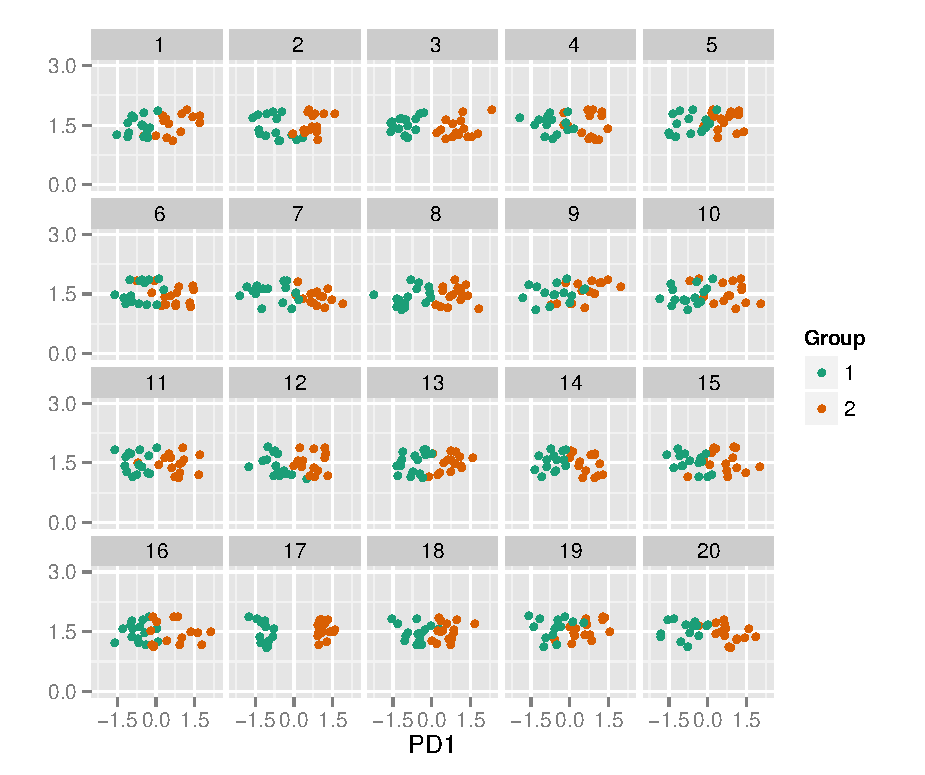
\includegraphics{lineup-20-real-1-17-rev.pdf}}
       \caption{Lineup  ($m=20$) from treatment with $p = 20$, separation = Yes and $d = 1$. The subjects were asked to identify the plot with the most separated colors. Can you identify the observed data plot? The solution to the lineup is provided in the Appendix. }
     \label{fig:test_category_1d}
\end{figure}


 
\begin{figure}[hbtp]
%   \centering
       \scalebox{1.00}{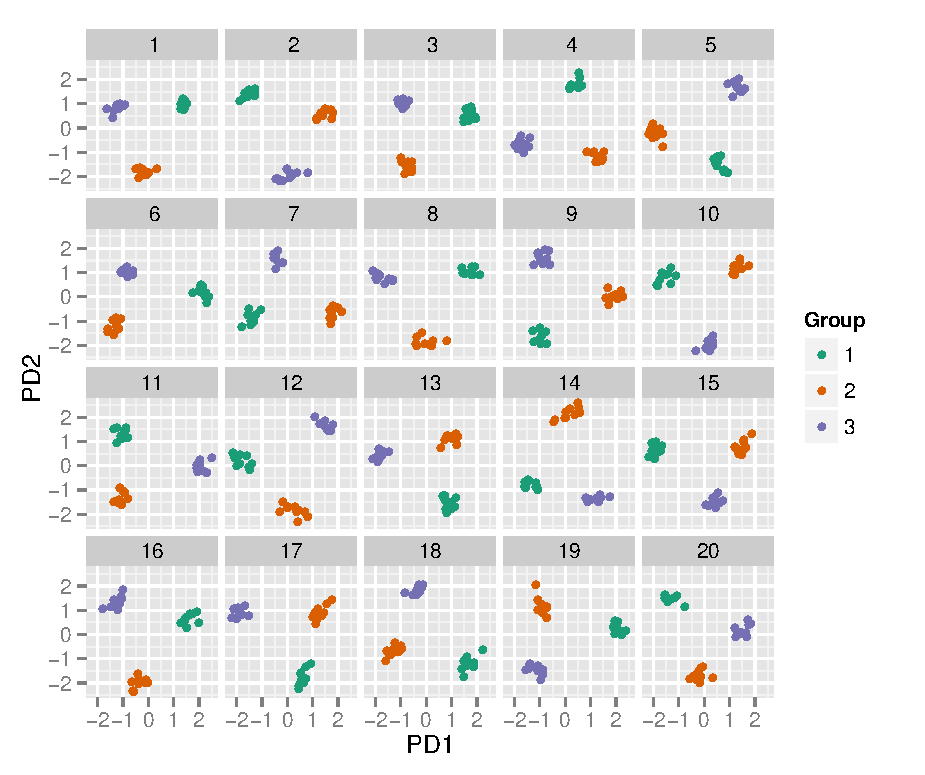
\includegraphics{lineup-100-noise-2-20-rev.pdf}}
       \caption{Lineup  ($m=20$) from treatment with $p = 100$, separation = No and $d = 2$.The subjects were asked to identify the plot with the most separation between the colored groups. Can you identify the observed data plot? The solution is provided in the Appendix. }
       \label{fig:test_category}
\end{figure}

%\ppp

\subsection{Data collection}

Subjects  for the experiment were recruited through Amazon's Mechanical Turk  \citep{turk}. 
%Amazon's Mechanical Turk is a medium that enables researchers to use human intervention to do tasks which the computers are unable to perform currently. In exchange of their efforts, the subjects were paid, not substantially, but on the scale of the minimum wage of the USA.  
Each subject was shown a block of ten lineups. They were asked to identify the plot which has the most separation between the colored groups. Their response was recorded along with a reason for their choice of the plot and the level of confidence they have in their decision.  Gender, age, educational level and the geographic location of each subject were also noted. In total, 1137 lineups were evaluated by 103 subjects, from different locations across the globe. 

%\subsection{Data cleaning}

Each subject was given a very easy lineup (a lineup with $p = 10$ dimensions with some real separation) in the block of ten. Data from subjects who failed to give a correct response to this lineup are removed from the study. If their response to this lineup was correct, data for this lineup was removed but responses for the remaining nine were kept for analysis. *** This produced XXX lineups evaluated by XXX subjects for analysis.


\section{Results} \label{sec:results}

\subsection{Effect of experimental factors} \label{effects}

We would expect that subjects are correct more often when there is real separation and that as dimension increases, correctness decreases. This is indeed the case, as illustrated by Figure \ref{suc-rate-glm}. The proportion correct is plotted against the different levels of dimension faceted by the levels of separation and projection. The 3 different dots for each level shows the 3 lineup replicates for each level combination of the factors. In a few cases, the dots overlap as the proportion correct is same for the replicates. For example, when projection = 1D, dimension = 100 and separation = No, the proportion correct is 0 for all the replicates and hence a single dot is shown. The line shows the fitted fixed effects from a logistic regression model fitted to the data. The success rate is higher for low dimension, and decreases as dimension increases, for real separation for both 1D and 2D projections. For noise data, the success rate is flat across dimension. There also appears to be increasing variance as dimension increases. Interestingly, the success rate is higher even at $p = 100$ for data where separation exists than for pure noise.

\begin{figure}[ht]
%\begin{figurehere}
   \centering
       \scalebox{0.6}{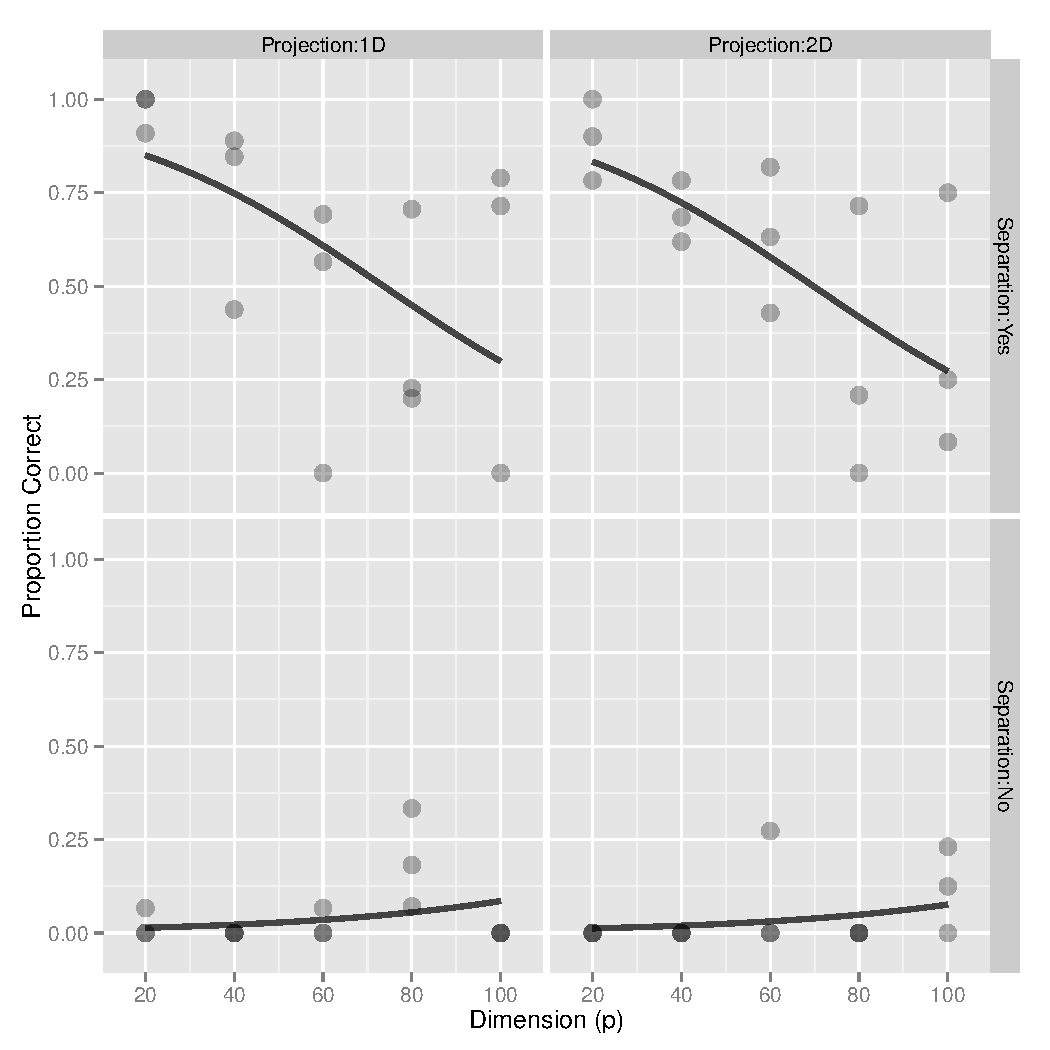
\includegraphics{suc-rate-rep-int-glm-rev.pdf}}
%        \scalebox{0.80}{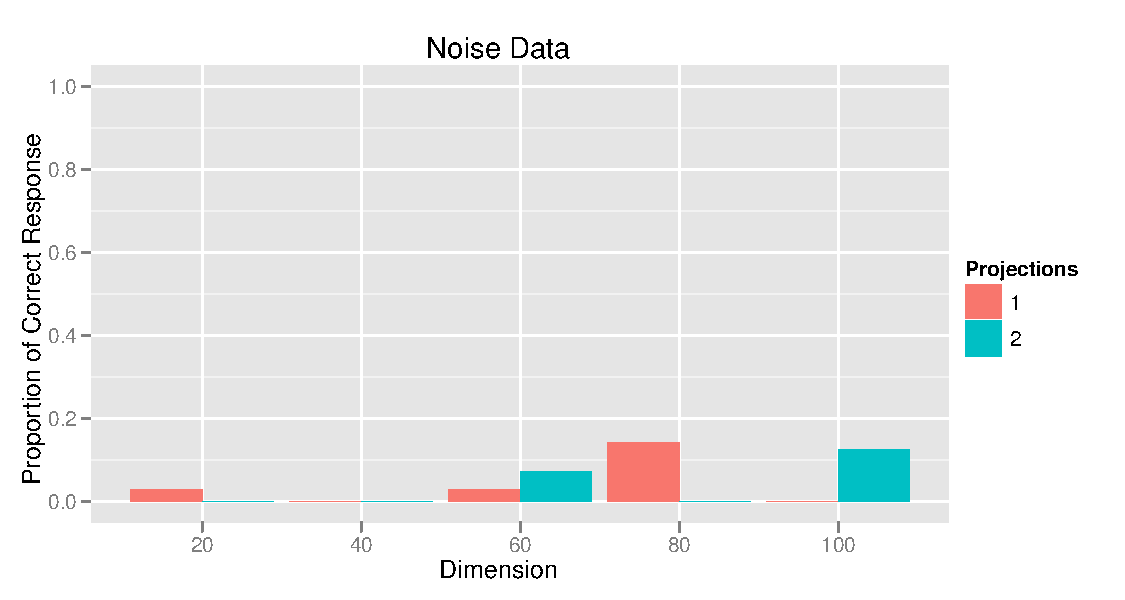
\includegraphics{result-noise.pdf}}
      \caption{Proportion of correct response against dimension faceted by projection and separation. The three points represents the three replicates for each treatment level. A fixed effects logistic regression model is overlaid on the points. It can be seen that the success rate decreases as dimension increases for data with real separation. When the data is purely noise data, the success rate is flat across dimensions. The success rate does not change with projection.  Even with $p = 100$ subjects more accurately picked the separation more often than would be by chance. }
       \label{suc-rate-glm}
\end{figure}

Table \ref{params} shows the estimates of the parameters from the fixed effects logistic regression model, the standard errors and the corresponding $p$-values. We observe that the $p$-values corresponding to dimension and presence of real separation is very highly significant. The interaction term is also significant. But the $p$-value corresponding to the projection is high, which suggests that the difference between 1D and 2D projections is not significant at the 5\% level of significance. One of our concerns with the 2D projections is that the rotation of the group was not adjusted, and that this might diminish the subjects ability to identify the observed data plot. The lack of significant difference between 1D and 2D results suggest that the lack of adjustment was not important. The slope of the covariate dimension is different when there is separation or not. When the observed data plot has real separation, the ability to detect it decreases with dimension.

\begin{table}[ht]
\begin{center}
\caption{Table summarizing results of experiment. Columns correspond to the estimate, the standard error and the $p$-value of the parameters used in logistic regression model. As dimension ($p$) increases, detection of separation decreases. Subjects can detect the separation if it exists even when $p = 100$. Subjects were equally good in 1D or 2D projections.}
\vspace{0.15cm}
\begin{tabular}{r|rrr}
\hline
  \hline
 Parameters & Estimate & Std. Error  & $p$-value \\ 
  \hline
Intercept  & 2.381 & 0.278  & 0.000 \\ 
  dimension($p$) & $-$0.032 & 0.004  & 0.000 \\ 
  separation = No & $-$7.097 & 0.911  & 0.000 \\ 
  projection = 2D & $-$0.127 & 0.181  & 0.483 \\ 
  separation:dimension & 0.056 & 0.011 & 0.000\\
   \hline
\end{tabular}
\label{params}
\end{center}
\end{table}

The effect of demographic variables on the proportion correct was also studied. The effects of education, age and gender were insignificant. 

%\subsection{Does rotation in the 2D projections affect the responses?}

%The 1D projections are plotted in a lineup (Figure \ref{fig:test_category_1d}) making the adjustment that the group with the lower values of projection are always considered to be group 1. So the orientation of the groups does not affect the response of the subjects. But in case of 2D projections, the groups are rotated in a different way in each plot in the lineup (Figure \ref{fig:test_category}) which may influence the response of the subjects. We can check if the rotation in the 2D projections does effect the performance. Since the 1D projections are adjusted, the lineups of the 1D projections are used as a control and the responses for the 1D and 2D projections are compared. Figure \ref{suc-rate-glm} shows that there is not much of a difference between the 1D and 2D projections both in presence and absence of real separation. This is also verified in Table \ref{params} where the effect of the projections is not significant at 5\% level.  

%\newpage

\subsection{Time taken to respond}

We would expect that the amount of time taken to respond will increase with the difficulty of identifying the observed data plot in a lineup. Figure \ref{time-taken} shows the time taken in seconds to respond (on a log scale) by dimension and projection. Color indicated separation or not. The line shows the trend over dimension. Bootstrap resampling bands (\cite{buja:2005}) are also drawn for each colored lines. Notice that,  when the data has some real separation (green), as the dimension increases, subjects take more time to respond to the lineups. But when the data is purely noise (brown), the increase of dimension does not have any effect on the time. This suggests that as the number of dimensions increases, it becomes harder to spot the observed data plot among the null plots. On the other hand, the difficulty of spotting the observed data plot for a data with purely noise does not vary with dimension. It can also be seen that the time taken when the data is purely noise is overall higher than the time taken when the data has some real separation. The bootstrap resampling band suggests that as dimension increases, the difference between time taken for data with separation and without separation decreases. 



\begin{figure*}[hbtp]
%\begin{figurehere}
   \centering
       \scalebox{0.7}{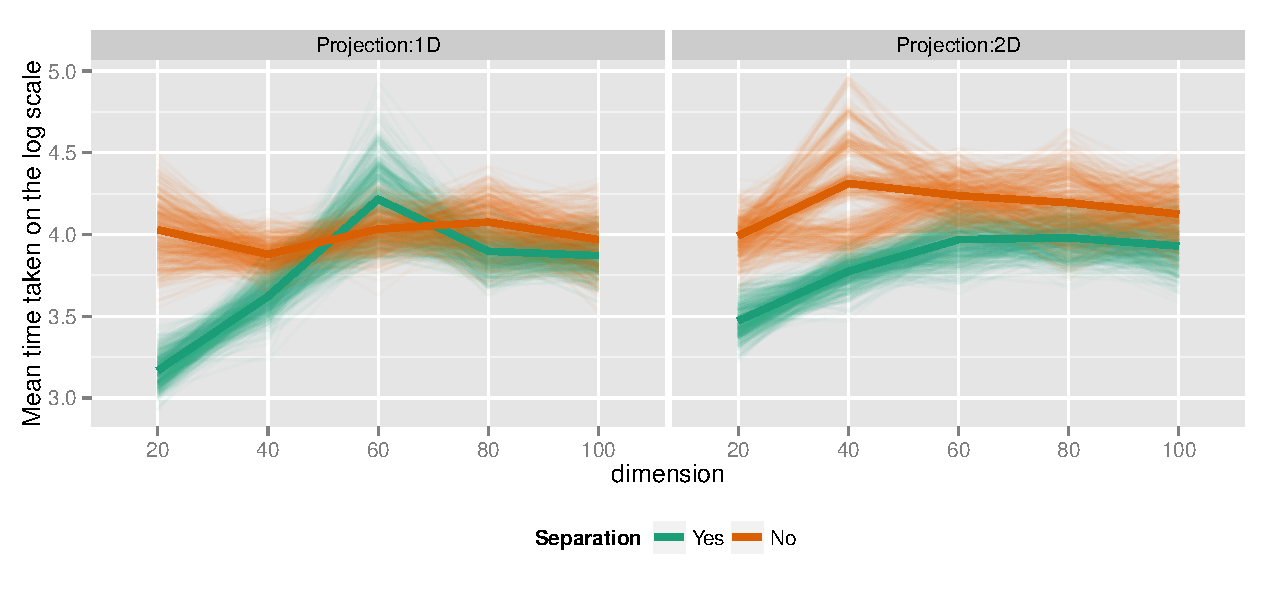
\includegraphics{time-taken-log-bands-1.pdf}}
%        \scalebox{0.80}{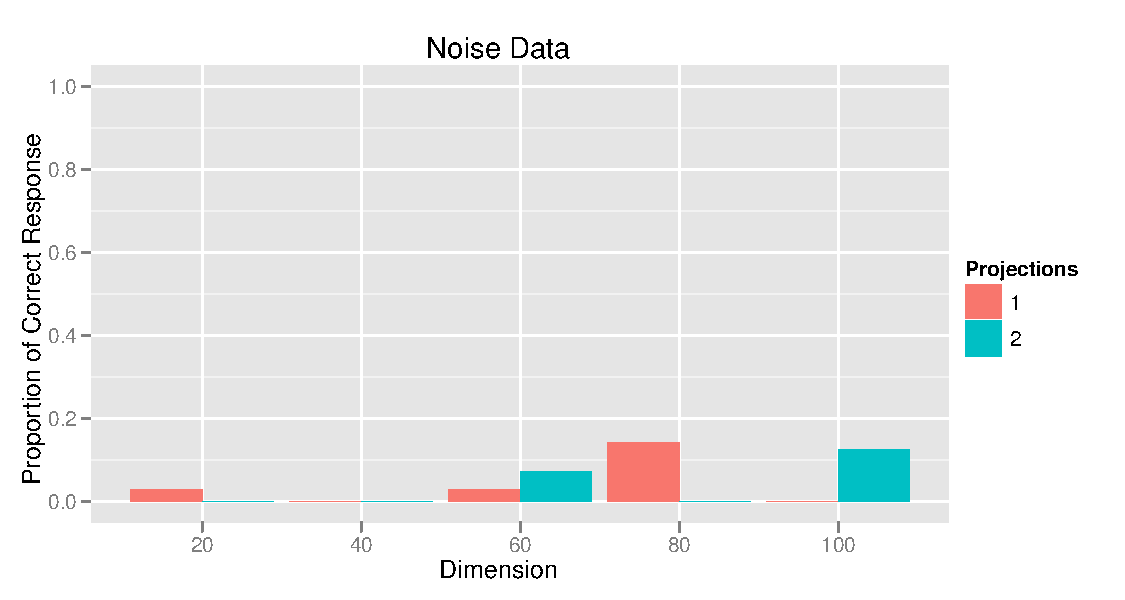
\includegraphics{result-noise.pdf}}
      \caption{Time taken in seconds to respond on log scale against dimension colored by separation and faceted by projection. A line shows the trend over dimension for each separation within projection. Bootstrap resampling bands are drawn for each colored lines. Time taken to respond is higher when the data has no separation. Also as dimension increases, the time to answer when there is separation is equal to the time taken when there is no separation. }
       \label{time-taken}
\end{figure*}

\subsection{What affects decisions?}

\normalsize

Figure \ref{sep} examines the subjects choices in detail. The relative frequency of picks of each plot in the lineup is plotted against a measure of average separation between groups. Each cell of this figure shows data from one of the lineups used in the study, 60 in total. Each ``pin'' represents a plot in a lineup, so each cell here has 20 pins, indicating the frequency that the plot was chosen. Red represents the observed data plot. Two separate figures are made for the two projections. The top three rows correspond to data containing real separation between the groups, and for the bottom three rows all of the data is purely noise. Columns indicate dimension ($p$). Replicates are in different rows. The taller the pin the more often that particular plot is chosen from the lineup. We asked subjects to pick the plot where the groups are most separated, and this is effectively what they picked. The plot in each lineup with the largest average separation tends to have the highest frequency. This is more obvious when there is real separation, and also when dimension is small, but it is also seen in the lineups containing pure noise data. This is reassuring -- that subjects did well at detecting the biggest difference.  
%For some of the lineups though, the choices are a little surprising, for example separation = No, dimension = 60, rep = 2, projection = 2D. Investigating these lineups further may reveal why this is. (See supplementary material).

\begin{figure}[htbp]
\centering
\mbox{\subfigure[For Projection:1D]{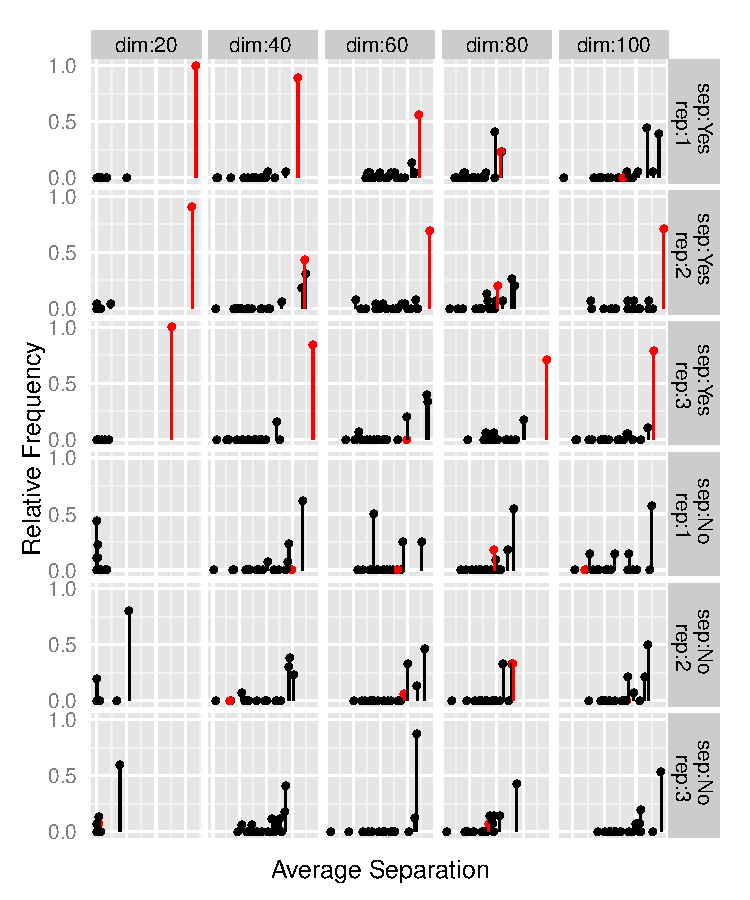
\includegraphics[width=3in]{avg-sep-1.pdf}}\quad
\subfigure[For Projection:2D]{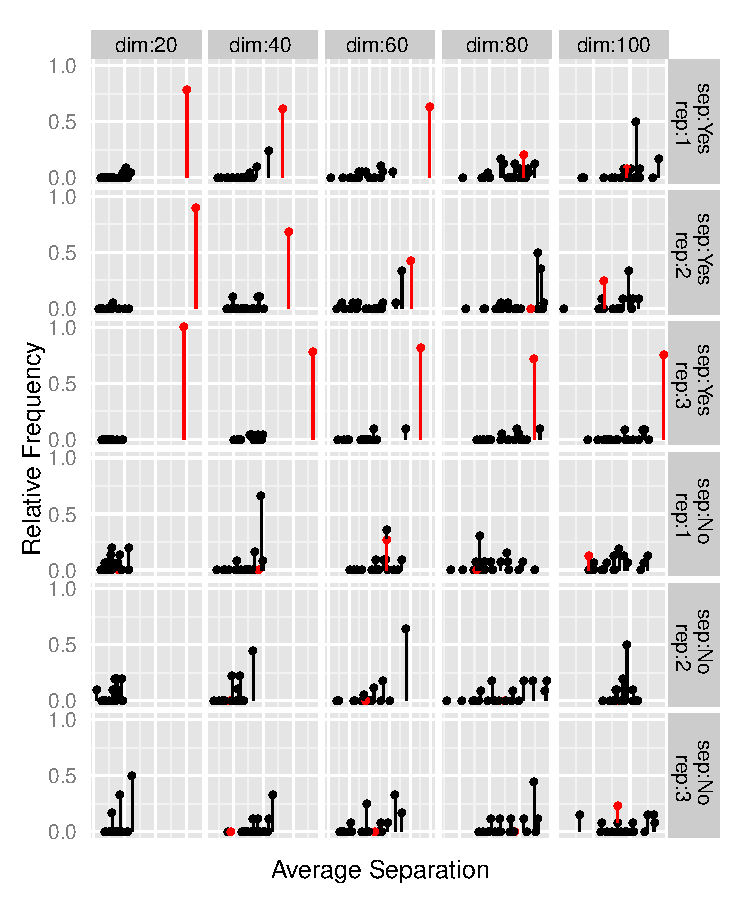
\includegraphics[width=3in]{avg-sep-2.pdf} }}
\caption{Comparing the choices that subjects make for each lineup. Relative frequency of plots chosen against a measure of the average separation between groups, the larger the value the more separated are the groups. Each cell here shows the data for one of the lineups used in the experiment, 60 in total, and each ``pin'' represents a plot in the lineup, 20 for each lineup. Red indicates the observed data plot. Subjects are asked to pick the plot in the lineup where the groups are the most separated, so we would expect that more subjects would pick the plots with the largest average separation. In general, this happens, the tallest pins are in the right of each cell. The top three rows show the results for the data with separation, so the observed data plot (red) is typically the pin on the very left of the cell, less so for the higher dimensions which are the cells at right. Figure (a) shows 1D projections and Figure (b) shows for 2D projections. There is not much difference between the two figures. } 
\label{sep}
\end{figure}

\subsection{How do the null plots affect choices?}

We have learned that subjects tend to pick the plot in the lineup that exhibits the most separation.  Because visual inference only allows for a finite (small) number of comparisons against the sampling distribution, the influence of the null plots in the lineup on the observer's choice is important. If any null plot has a strong signal, subjects may choose this plot over the observed data plot. To gauge the influence of the null plots, we first calculate the average separation between the clusters in each plot of the lineup. For each lineup we then calculate the difference between the maximum average separation of the null plots and the average separation for the observed data plot for each lineup. Figure \ref{null} examines the influence of the null plots on this pick. The proportion correct and mean time taken in seconds are plotted against difference. The vertical line is a reference line where the difference is 0; the value at which the observed data plot has the same signal as the most extreme null plot. The points to the right of the line should indicate easier lineups and those to the left indicate more difficult lineups in the sense that the null plots have more signal than the observed data plot. We can see that as the difference increases, the success rate increases and also time taken to choose decreases, suggesting easier lineups. More details on the measurement of the influence of the null plots are available in \cite{roychowdhury:2012}).

\begin{figure}[htbp]
\centering
\subfigure[For Projection:1D]{
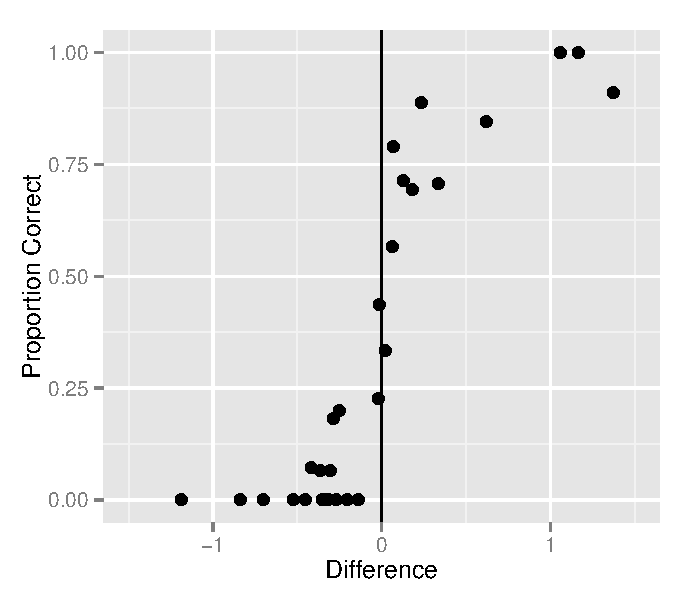
\includegraphics[width=3in]{suc-diff-avg-sep-1.pdf}
}
\subfigure[For Projection:2D]{
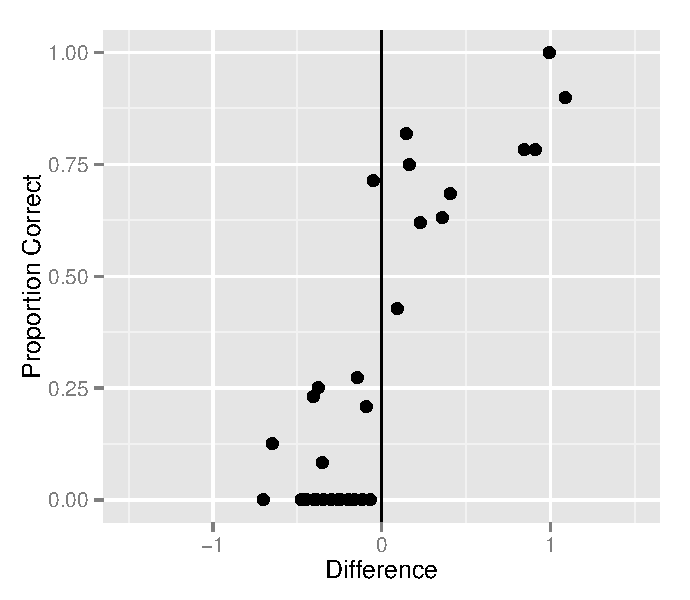
\includegraphics[width=3in]{suc-diff-avg-sep-2.pdf}
}
\subfigure[For Projection:1D]{
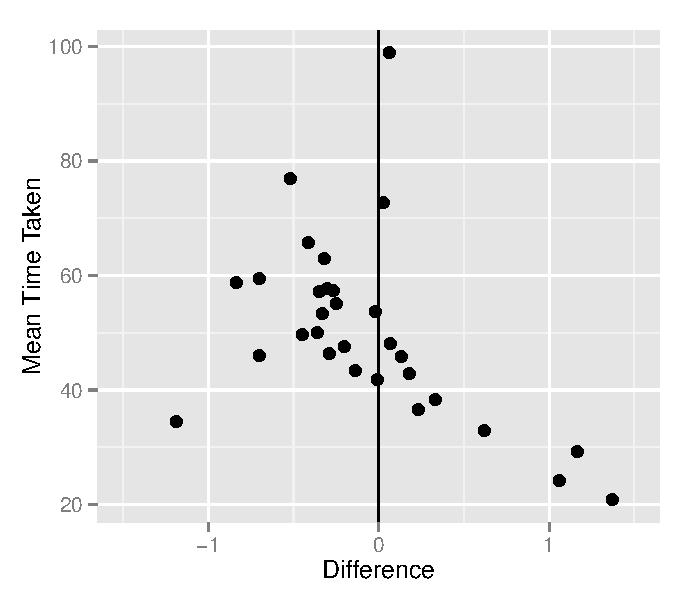
\includegraphics[width=3in]{mtime-diff-avg-sep-1.pdf}
}
\subfigure[For Projection:2D]{
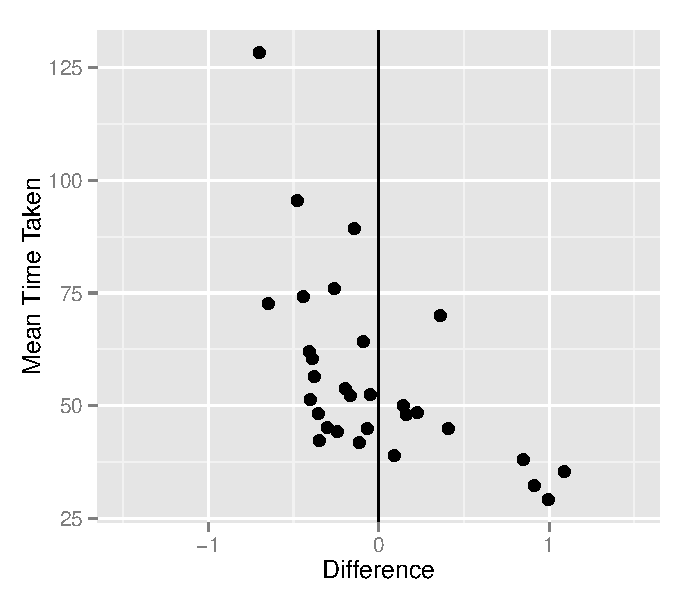
\includegraphics[width=3in]{mtime-diff-avg-sep-2.pdf} 
}
\caption{Proportion of correct response and mean time taken to respond in seconds are plotted against the difference for 1D and 2D projections separately. The difference is between maximum separation of all the null plots and separation of the observed data plot for each lineup for 1D projections but for 2D projections the difference is based on the average separation between the groups. The vertical line represents difference equal to 1 when the average separation of the observed data plot is equal to the maximum average separation of the null plots for 2D projection. The points left to the line indicates a difficult lineup in the sense that at least one of the null plots had a lower average separation value than the observed data plot. (a) and (b) As difference increases, success rate increases. (c) and (d) As difference increases,  mean time taken decreases indicating that the subjects have an easier time in identifying the observed data plot. }
\label{null}
\end{figure}

\section{Conclusions}

This paper examined the application of visual inference to HDLSS data. From the results, it is clear that people can detect real separation from pure noise  up to a reasonably high dimension, for 1D and 2D projections. This suggests that visual inference may be effective for improving the understanding of the emptiness of space in HDLSS data. That is, a 1D or 2D projection of HDLSS data,  as provided by LDA, for example, will likely look separated purely due to this emptiness. Visual inference makes this clearer and provides a calibration for reading the separation. Visual inference methods shows that the projection pursuit optimization procedure works well in \texttt{tourr} package. This technique can be used to test the convergence algorithm in any other method where the optimization procedure is involved like multidimensional scaling, PCA, independent component analysis (ICA) and local linear embeddings.

There are several natural next steps for this research. One is to examine the possibility of using visual inference to obtain confidence bands for the value of $p$, where separation is certain, for fixed sample size and dimension, particularly if a component of real separation is included. Another direction is to build metrics to quantify the difficulty of a lineup and the influence that null plots have on identifying the data plot. In a future study, the effect of short fixed time responses will be studied.



\section*{Acknowledgement}
%
This work was funded by National Science Foundation grant DMS 1007697. All figures were made using the R \citep{r} package ggplot2 \citep{hadley:2009}.

%\bibliographystyle{plainnat}
\bibliographystyle{spbasic}
%%\bibliographystyle{ieeetr}
\bibliography{references}

\section*{Appendix}

\subsection*{Solution}
\begin{itemize}
\item The solution to the lineup at Figure \ref{lineup} is Plot 16. 
\item The solution to the lineup at Figure \ref{fig:test_category_1d} is Plot 17.
\item The solution to the lineup at Figure \ref{fig:test_category} is Plot 20.
\item The solution to the lineup at Figure \ref{toth_lineup} is Plot 8.

\end{itemize}

\subsection*{Choice of dimensions} \label{sec:theory}

The experiment is set up with the 3 factors separation, dimension and projection dimension. To decide on the levels of dimension to use, we considered the distribution of the absolute difference of the sample group means, for data with two groups, no separation and projection dimension $d=1$. The same levels are used for data with 3 groups, $d=2$, and for data with separation. 

Let ${\blX}_{ij}$ denote the $j$-th observation in the $i$-th group where $j = 1, \dots, n; i=1, ..., g$. The ${\blX}_{ij}$'s are random noise, generated by drawing samples from a standard normal distribution. For this experiment, $g = 2$  and $n = 15$. The difference between the group means is given by $\overline{\mbox{X}}_{1.} - \overline{\mbox{X}}_{2.}$% and $$\overline{\mbox{X}}_{1.} - \overline{\mbox{X}}_{2.} \sim \hbox{Normal}(0, 1/n_1 + 1/n_2)$$ i.e. 
and $$\overline{\mbox{X}}_{1.} - \overline{\mbox{X}}_{2.} \sim \hbox{Normal}(0, 2/15)$$ Let 
$\mbox{U} = |\overline{\mbox{X}} _{1.} - \overline{\mbox{X}}_{2.}|$ 
where $\mbox{U} \sim \hbox{Half Normal}$ with scale parameter $ \sigma = \sqrt{2/15}$.
The expectation and the variance of $\mbox{U}$ are 
$E(\mbox{U} ) = \sigma \sqrt{2/\pi}$ and 
$Var(\mbox{U}) = \sigma^2 (1 - 2/\pi)$, respectively.

For $p$ dimensions, consider $p$ independent samples from the same distribution,  denoted as $${\blU}_m = |\overline{{\blX}}_{m1.} - \overline{{\blX}}_{m2.}|, ~~~ m=1, ..., p$$ where ${\blX} _{mij}$ is the $j$-th observation in the $i$-th group for the $m$-th dimension. The difference between the two group means projected into one dimension, is the sum over $p$ dimensions of the absolute difference between the means: $$\mbox{U}  = \sum_{m=1}^p {\blU}_m = \sum_{m=1}^p |\overline{{\blX}}_{m1.} - \overline{{\blX}}_{m2.}| $$ and by independence it follows that

$$\hbox{E}(\mbox{U}) = p \sigma \sqrt{2/\pi}, ~~~ 
\hbox{Var}(\mbox{U}) = p \sigma^2 (1 - 2/\pi)$$

\noindent Thus we expect to find this amount of separation between the projected sample means, for data sampled from populations with the same means.

Now consider data where there is some separation (equal to $2c)$ between the population means:

$${\blZ}_{1j} \sim \hbox{Normal}(-c, 1) $$
$${\blZ}_{2j} \sim \hbox{Normal}(c, 1) $$ 
giving $\overline{\mbox{Z}}_{1.} - \overline{\mbox{Z}}_{2.} \sim \hbox{Normal}(2c, 2/15)$. Then define $\mbox{Z}  = |\overline{\mbox{Z}}_{1.} - \overline{\mbox{Z}}_{2.}|$ where ${\mbox{Z}} \sim \hbox{Folded Normal Distribution}$ with scale parameter $ \sigma = \sqrt{2/15}$.  The expectation and the variance of $\mbox{Z}$ can be calculated to be:

$$\hbox{E}(\mbox{Z}) = \sigma \sqrt{2/\pi} \exp(- 2c^2/\sigma^2) + 2c[1 - \Phi(-2c/\sigma)]$$
$$\hbox{Var}(\mbox{Z}) = 4c^2 + \sigma^2 - (E(\mbox{Z}))^2$$

Suppose that only one of the $p$ dimensions is simulated from this distribution, and all of the rest are simulated from populations having identical means. Define $\mbox{V}$ as the sum of the absolute differences of the mean with one dimension of real separation as $$\mbox{V} = \sum_{m=1}^{p-1} \blU_m + {\blZ}$$ Then, by independence, it follows that:

$$\hbox{E}(\mbox{V}) = (p - 1) \sigma \sqrt{2/\pi} + \sigma \sqrt{2/\pi} \exp(- 2c^2/\sigma^2) + 2c[1 - \Phi(-2c/\sigma)]$$
$$\hbox{Var}(\mbox{V}) = (p - 1)\sigma^2 (1 - 2/\pi) + 4c^2 + \sigma^2 - \left( \sigma \sqrt{2/\pi} \exp(- 2c^2/\sigma^2) + 2c[1 - \Phi(-2c/\sigma)]\right)^2$$

In this experiment, $c = 3$ and $\sigma^2 = 2/15$. Therefore,
$$\exp(- 2c^2/\sigma^2) \approx 0 \qquad \hbox{and} \qquad \Phi(-2c/\sigma) \approx 0$$
Hence,
$$\hbox{E}(\mbox{V}) = (p - 1) \sigma \sqrt{2/\pi} + 6$$
$$\hbox{Var}(\mbox{V}) = (p - 1)\sigma^2 (1 - 2/\pi) + \sigma^2$$
As dimension $p$ increases for a fixed $n$, the spread of both U and V increases by a factor of $p$. The means of U and V also increase with a factor of $p$ but the expected value of the difference between U and V stays constant and is independent of dimension ($p$). 
%\begin{equation}
$$\hbox{E} (\mbox{V} - \mbox{U}) = (p - 1) \sigma \sqrt{2/\pi} + 6 - p \sigma \sqrt{2/\pi} = 6 - \sigma \sqrt{2/\pi}$$
%\end{equation}

Two $p$-dimensional datasets are generated with 30 observations in each dimension. The datasets are then divided into two groups with 15 observations in each group. For one set, data is obtained from random noise and hence there is no real separation between the two groups. But for the other set, one dimension among these $p$ is adjusted so that the data have some real separation between the groups in that dimension. The absolute difference of the means for each group in each of these $p$ dimensions is considered for both datasets. The absolute difference is considered as we are concerned with projections. These absolute differences between the groups are then summed over all the dimensions to obtain the absolute difference of means for the data. This process is repeated 1000 times. These 1000 sum of absolute differences are then plotted for the different values of $p$.
 
Figure \ref{fig:dimen} shows the distribution of sum of absolute difference of means for data with and without separation for different dimensions. The distributions of data with and without separation are shown in brown and green respectively. The area of the distribution of pure noise which is above the 5th percentile of the distribution of data with separation is shown in dark blue and it can be seen that the dark blue region increases with dimension ($p$). This indicates that as dimension increases, the distributions of data with or without separation gets closer. Hence it gets harder to detect real differences with higher dimensions. Fixing the area of the dark blue region and calculating the dimensions to obtain the required region provides the choice of levels of dimension used in the experiment. More details are provided in Section \ref{sec:theory}. 

\begin{figure}[hbtp]
%\begin{figurehere}
   \centering
       \scalebox{0.70}{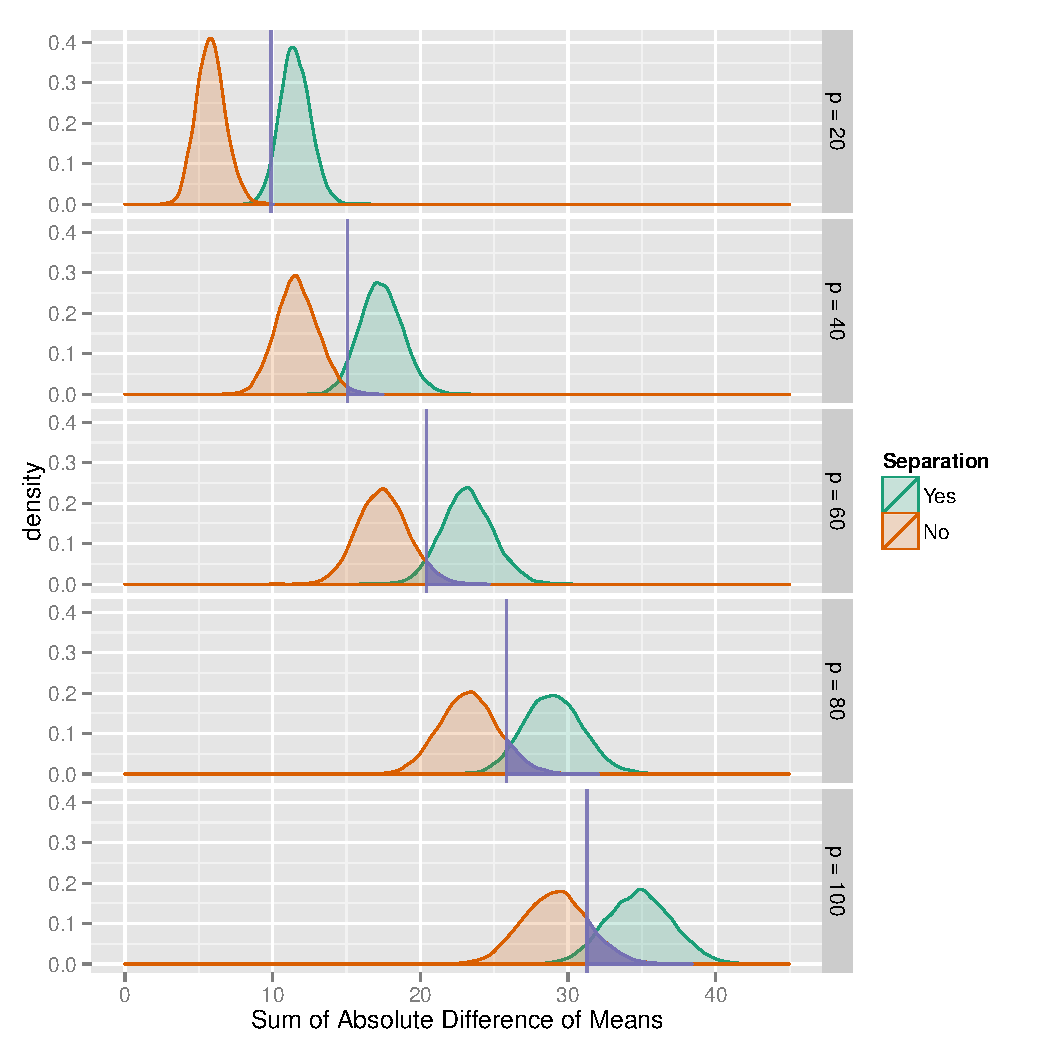
\includegraphics{sum-noise-real-2-rev.pdf}}
       \caption{Plot showing the distribution of the sum of absolute difference of means for data with and without separation for different dimensions. The distributions of data with real separation (V) and purely noise data (U) are shown in brown and green respectively with the dark blue line showing the 5th percentile of V. The dark blue area shows the area of U which is greater than the 5th percentile of V. The dark blue region ($\delta$) increases as dimension ($p$) increases. }
     \label{fig:dimen}
%\end{figurehere}
\end{figure}


Figure \ref{fig:dimen} illustrates this phenomenon. The distributions of data with separation (V) and without separation (U) are shown in red and blue respectively. As dimension ($p$) increases, the spread of both the distributions increases while the means are equally apart. As a result, the common region between the distributions increases, indicating the chance of obtaining a random separation for purely noise data increases with dimension($p$). A 5\% error is allowed and the area of the distribution of U greater than the 5th percentile of V is considered and we call this $\delta$. In Figure \ref{fig:dimen}, $\delta$ is indicated by the dark blue region. Mathematically, 

$$\hbox{P}[\mbox{U} > \mbox{V}_{\alpha}] = \delta$$ where $\mbox{V}_{\alpha}$ is the $100\alpha$-th percentile of V, where $\alpha = 0.05$.  Dimension $p$ is calculated for fixed values of $\delta$. The various values of $\delta$ are chosen such that the distributions has no separation ($\delta \approx 0$) or has 1\%, 5\%, 10\% and 20\% common region. For each value of $\delta$, the procedure is repeated 100 times and Table \ref{tab:dimen} shows the summaries of the dimension ($p$) for each value of $\delta$.

\begin{table}[htbp]
\begin{center}
\caption{Numerical summaries of dimension $p$ for each value of $\delta$. As the common region $\delta$ increases, the median dimension required to obtain the region increases.}
\begin{tabular}{rrrr}
  \hline
  \hline
  $\delta$ & Median & 5th percentile & 95th percentile \\
  \hline
  0.0000001 & 24 & 19 & 28 \\
      0.01 & 41 & 38 & 44\\
   0.02 & 61 & 56 & 64 \\
     0.1 & 77 & 72 & 81\\   
     0.2 & 106 & 99 & 112\\ 
      \hline
\end{tabular}
\label{tab:dimen}
\end{center}
\end{table}


\end{document}
